% =============================================================================
% Module 3: Cosmological Distances
% =============================================================================
% Sources: Carroll Ch. 8 (FRW cosmology, Friedmann equations);
%          Congdon & Keeton Ch. 3.5 (cosmological distances for lensing);
%          Narayan & Bartelmann Sec. 2.1.3;
%          Weinberg, Cosmology (2008) Ch. 1
% Mathematica: ../Mathematica/03_Cosmological_Distances/
% =============================================================================

\chapter{Cosmological Distances}
\label{ch:cosmological_distances}

\begin{quote}
\textit{Not only does God definitely play dice, but He sometimes confuses us by
throwing them where they can't be seen.}
\hfill --- Stephen Hawking, \textit{Does God Play Dice?} (public lecture, 1999)
\end{quote}

\noindent
Gravitational lensing is inherently a cosmological phenomenon: the lens
and source are typically at redshifts $z \sim 0.1$--$3$, separated by
distances of order gigaparsecs.  To connect the physical deflection angle
$\alphahat = 4\Gnewton M / (\speedoflight^2 b)$ derived in Modules~1e
and~2 to observable image positions on the sky, we need a precise
definition of ``distance'' in an expanding universe.  Unlike in Euclidean
space, there is no single notion of distance in cosmology: the
\textit{angular diameter distance} (relevant for angles), the
\textit{luminosity distance} (relevant for fluxes), and the
\textit{comoving distance} (relevant for volumes) are all distinct.

This module develops the full framework of cosmological distances from
first principles.  In Part~A we derive the Friedmann--Lema\^{i}tre--Robertson--Walker (FLRW)
metric from the cosmological principle, compute the Christoffel symbols
and curvature tensors for this metric using the tools from Module~1b,
and plug into Einstein's equations with a perfect-fluid
stress-energy tensor to obtain the \textbf{Friedmann equations} ---
the dynamical equations governing the expansion of the universe.  In
Part~B we define the various distance measures, derive the key distance
ratios that enter the lens equation, and highlight the counterintuitive
\textit{non-monotonicity} of the angular diameter distance, which turns
over at $z \sim 1.6$ for the concordance cosmology.

\medskip
\noindent
\textbf{Companion Mathematica files:}
\begin{itemize}[nosep]
    \item \mathlink{03_Cosmological_Distances/friedmann_equations.wl}{friedmann\_equations.wl}
          --- symbolic computation of Christoffel symbols and curvature
          tensors for the FRW metric, derivation of the Friedmann equations,
          scale factor solutions, cosmological distance calculations,
          and figure generation
    \item \mathlink{03_Cosmological_Distances/cosmological_distances.nb}{cosmological\_distances.nb}
          --- interactive notebook with sliders for $\Omegam$,
          $\OmegaL$, $\Hubble$ showing how distance--redshift relations
          change; lensing geometry calculator
\end{itemize}


% #########################################################################
% PART A: THE FRW METRIC AND FRIEDMANN EQUATIONS
% #########################################################################

\section*{Part A: The FRW Metric and Friedmann Equations}
\addcontentsline{toc}{section}{Part A: The FRW Metric and Friedmann Equations}

% =====================================================================
\section{The Cosmological Principle}
\label{sec:cosmological_principle}

Modern cosmology rests on the \textbf{cosmological principle}: on
sufficiently large scales ($\gtrsim 100$~Mpc), the universe is
\textit{spatially homogeneous} (the same at every point) and
\textit{spatially isotropic} (the same in every direction).  These two
symmetry assumptions are supported by:
\begin{itemize}
    \item The near-perfect isotropy of the cosmic microwave background
          (CMB), which is uniform to one part in $10^5$ across the sky.
    \item The large-scale distribution of galaxies, which becomes
          statistically uniform on scales $\gtrsim 100$~Mpc, as shown
          by surveys such as SDSS, 2dFGRS, and DESI.
\end{itemize}

\begin{remark}
Homogeneity and isotropy constrain only the \textit{spatial} geometry of
the universe at each instant.  The universe is manifestly \textit{not}
homogeneous in time: it was denser and hotter in the past.  The metric
is therefore allowed to have time-dependent coefficients (the scale
factor), and it is this time dependence that encodes the expansion
history.
\end{remark}

The mathematical consequence of the cosmological principle is powerful:
the spatial part of the metric must be a maximally symmetric
3-dimensional Riemannian manifold.  By a classic theorem in differential
geometry (see Carroll Secs.~3.9 and~8.2), maximally symmetric $n$-dimensional
spaces have $n(n+1)/2$ Killing vectors, and there are exactly three
possibilities for $n = 3$: positive curvature (the 3-sphere $S^3$),
zero curvature (flat $\mathbb{R}^3$), or negative curvature (the
3-hyperboloid $H^3$).  These are characterized by a single parameter,
the \textbf{spatial curvature constant} $k$:
\begin{equation}
    k = \begin{cases}
    +1 & \text{positive curvature (closed, finite volume)} \\
    \phantom{+}0 & \text{zero curvature (flat, infinite volume)} \\
    -1 & \text{negative curvature (open, infinite volume)}
    \end{cases}
    \label{eq:k_values}
\end{equation}


% =====================================================================
\section{The Robertson--Walker Metric}
\label{sec:rw_metric}

Combining the cosmological principle with the requirement that spacetime
be described by a Lorentzian 4-metric, the most general metric takes the
\textbf{Robertson--Walker (RW)} form (Carroll eq.~8.43; Congdon \& Keeton
eq.~3.123a):
\begin{equation}
    \boxed{
    ds^2 = -\speedoflight^2\, dt^2
    + a^2(t) \left[\frac{dr^2}{1 - kr^2}
    + r^2 \bigl(d\theta^2 + \sin^2\!\theta\, d\phi^2\bigr)\right]
    }
    \label{eq:rw_metric}
\end{equation}
where:
\begin{itemize}
    \item $t$ is \textbf{cosmic time} --- the proper time measured by
          comoving observers (those at rest with respect to the Hubble
          flow).
    \item $a(t)$ is the \textbf{scale factor}, a dimensionless function
          of time that encodes how distances between comoving observers
          change.  We adopt the convention $a(t_0) = 1$ at the present
          epoch.
    \item $r$, $\theta$, $\phi$ are \textbf{comoving coordinates} ---
          the coordinate labels assigned to comoving observers do not
          change as the universe expands.  The \textit{physical} distance
          between two comoving observers separated by coordinate distance
          $\Delta r$ is $a(t)\,\Delta r$, which grows with time if the
          universe is expanding ($\dot{a} > 0$).
    \item $k = -1, 0, +1$ is the spatial curvature parameter.
\end{itemize}

\begin{remark}
The metric~\eqref{eq:rw_metric} is purely \textit{kinematical}: it is
the most general metric consistent with homogeneity and isotropy, but
it tells us nothing about how $a(t)$ evolves.  The dynamics of $a(t)$
come from plugging this metric into Einstein's field equations, which we
do in the next sections to derive the Friedmann equations.
\end{remark}

It is often useful to write the spatial part of the metric using the
\textbf{comoving distance} $\chi$ defined by
\begin{equation}
    d\chi = \frac{dr}{\sqrt{1 - kr^2}} \,,
    \label{eq:comoving_distance_def}
\end{equation}
so that
\begin{equation}
    ds^2 = -\speedoflight^2\, dt^2
    + a^2(t)\left[d\chi^2 + S_k^2(\chi)\, d\Omega^2\right] ,
    \label{eq:rw_metric_chi}
\end{equation}
where $d\Omega^2 = d\theta^2 + \sin^2\!\theta\, d\phi^2$ and the
\textbf{transverse comoving distance} $S_k(\chi)$ is
\begin{equation}
    S_k(\chi) = \begin{cases}
    \sin\chi & k = +1 \\
    \chi     & k = 0 \\
    \sinh\chi & k = -1
    \end{cases}
    \label{eq:Sk}
\end{equation}


\begin{derivation}[From $d\chi = dr/\sqrt{1-kr^2}$ to $r = S_k(\chi)$]
Integrate from the origin: for $k = +1$, $\chi = \int_0^r dr'/\sqrt{1-r'^2}
= \arcsin r$, so $r = \sin\chi$; for $k = -1$, $\chi = \int_0^r
dr'/\sqrt{1+r'^2} = \operatorname{arcsinh} r$, so $r = \sinh\chi$; for $k=0$,
$r = \chi$ (check B9).  Substituting $r = S_k(\chi)$ into the angular part
$r^2 d\Omega^2$ gives eq.~\eqref{eq:rw_metric_chi}.
\end{derivation}

\begin{annotation}[Units trap: $k = \pm1$ makes $r$ and $\chi$ dimensionless]
With $k \in \{-1,0,+1\}$ and a dimensionless $a$ normalised to $a(t_0) = 1$,
the combination $kr^2$ forces $r$ (and $\chi$) to be measured in units of the
present curvature radius $R_0$.  To get a distance in Mpc for $k \neq 0$, restore
$R_0$: the transverse comoving distance is $D_M = R_0\,S_k(\chi/R_0)$ with $\chi$
now in Mpc, and $R_0 = (\speedoflight/\Hubble)/\sqrt{|\Omega_k|}$ (from the
definition of $\Omega_k$ below).  This is the form used in
eq.~\eqref{eq:Dds_general}.  For the flat case used throughout Parts~IV--V,
$S_k(\chi) = \chi$ and the issue disappears.
\end{annotation}

% =====================================================================
\section{Christoffel Symbols for the FRW Metric}
\label{sec:frw_christoffel}

To derive the Friedmann equations, we need the Christoffel symbols,
Ricci tensor, and Ricci scalar for the RW metric~\eqref{eq:rw_metric}.
We use the general functions developed in Module~1b
(\mathlink{01b_Differential_Geometry/christoffel_symbols.wl}{christoffel\_symbols.wl})
and verified symbolically in
\mathlink{03_Cosmological_Distances/friedmann_equations.wl}{friedmann\_equations.wl}.

The coordinates are $x^\mu = (t, r, \theta, \phi)$, and the nonvanishing
metric components are (reading off from eq.~\eqref{eq:rw_metric}):
\begin{align}
    g_{00} &= -\speedoflight^2 \,, &
    g_{11} &= \frac{a^2(t)}{1 - kr^2} \,, \nonumber \\
    g_{22} &= a^2(t)\, r^2 \,, &
    g_{33} &= a^2(t)\, r^2 \sin^2\!\theta \,.
    \label{eq:frw_metric_components}
\end{align}

Since this is a diagonal metric, we use the formulas from Module~1b
(Remark~\ref{rem:diagonal_shortcut}): for a diagonal metric with components $g_{aa}$ (no sum),
\begin{align}
    \christoffel{a}{b}{b} &= -\frac{1}{2g_{aa}}\, \partial_a g_{bb}
    \qquad (a \neq b) \,, \nonumber \\
    \christoffel{a}{a}{b} &= \frac{1}{2g_{aa}}\, \partial_b g_{aa}
    \qquad (\text{no sum on } a) \,.
    \label{eq:diagonal_christoffel}
\end{align}

The \textbf{nonvanishing Christoffel symbols} of the RW metric are
(Carroll eq.~8.44; verified in
\texttt{friedmann\_equations.wl}):

\medskip
\noindent\textbf{Time-space mixed:}
\begin{equation}
    \christoffel{0}{1}{1} = \frac{a\dot{a}}{\speedoflight^2(1-kr^2)} \,,
    \quad
    \christoffel{0}{2}{2} = \frac{a\dot{a}\, r^2}{\speedoflight^2} \,,
    \quad
    \christoffel{0}{3}{3} = \frac{a\dot{a}\, r^2 \sin^2\!\theta}{\speedoflight^2}
    \label{eq:christoffel_0ij}
\end{equation}
and their counterparts (mixed time--space, related by the symmetry $\christoffel{\rho}{\mu}{\nu} = \christoffel{\rho}{\nu}{\mu}$):
\begin{equation}
    \christoffel{1}{0}{1} = \christoffel{2}{0}{2}
    = \christoffel{3}{0}{3} = \frac{\dot{a}}{a}
    \label{eq:christoffel_i0j}
\end{equation}
where the dot denotes $d/dt$.

\medskip
\noindent\textbf{Purely spatial:}
\begin{align}
    \christoffel{1}{1}{1} &= \frac{kr}{1-kr^2} \,, &
    \christoffel{1}{2}{2} &= -r(1-kr^2) \,, \nonumber \\
    \christoffel{1}{3}{3} &= -r(1-kr^2)\sin^2\!\theta \,, &
    \christoffel{2}{1}{2} &= \frac{1}{r} \,, \nonumber \\
    \christoffel{2}{3}{3} &= -\sin\theta\cos\theta \,, &
    \christoffel{3}{1}{3} &= \frac{1}{r} \,, \nonumber \\
    \christoffel{3}{2}{3} &= \frac{\cos\theta}{\sin\theta} \,.
    \label{eq:christoffel_spatial}
\end{align}


\begin{derivation}[Four representative symbols from the diagonal formulas]
Only $g_{11}$, $g_{22}$, $g_{33}$ depend on $t$ (through $a^2$), $g_{11}$ depends
on $r$, $g_{22}$ on $r$, and $g_{33}$ on $r$ and $\theta$.  Every nonzero symbol
comes from one of these derivatives.
\begin{align*}
  \christoffel{0}{2}{2} &= -\frac{1}{2g_{00}}\,\partial_t g_{22}
    = -\frac{1}{2(-\speedoflight^2)}\,2a\dot a\,r^2
    = \frac{a\dot a\,r^2}{\speedoflight^2},\\
  \christoffel{2}{0}{2} &= \frac{1}{2g_{22}}\,\partial_t g_{22}
    = \frac{2a\dot a\,r^2}{2a^2r^2} = \frac{\dot a}{a},\\
  \christoffel{1}{1}{1} &= \frac{1}{2g_{11}}\,\partial_r g_{11}
    = \frac{1-kr^2}{2a^2}\cdot\frac{2kr\,a^2}{(1-kr^2)^2} = \frac{kr}{1-kr^2},\\
  \christoffel{1}{2}{2} &= -\frac{1}{2g_{11}}\,\partial_r g_{22}
    = -\frac{1-kr^2}{2a^2}\cdot 2a^2 r = -r(1-kr^2).
\end{align*}
The remaining nine follow the same two patterns.  The script checks all
thirteen against the general \texttt{computeChristoffel} and confirms there is
no fourteenth (checks B1a--b).  Note the $1/\speedoflight^2$ in
$\christoffel{0}{i}{i}$ and its absence in $\christoffel{i}{0}{i}$: the first
has an upper time index (divide by $g_{00} = -\speedoflight^2$), the second a
lower one.
\end{derivation}
\begin{exercise}
\label{ex:frw_christoffel}
Compute all nonvanishing Christoffel symbols of the RW metric by hand
using the diagonal metric formulas~\eqref{eq:diagonal_christoffel}.
Verify your results with
\mathlink{03_Cosmological_Distances/friedmann_equations.wl}{friedmann\_equations.wl},
which uses the general \texttt{computeChristoffel} function from
Module~1b.
\end{exercise}


% =====================================================================
\section{Ricci Tensor and Ricci Scalar}
\label{sec:frw_ricci}

From the Christoffel symbols, we compute the Riemann tensor
$\riemann{\rho}{\sigma}{\mu}{\nu}$, contract to obtain the Ricci tensor
$R_{\mu\nu} = R^\lambda_{\ \mu\lambda\nu}$, and then contract again
with the inverse metric to get the Ricci scalar $\ricciS = g^{\mu\nu}
R_{\mu\nu}$.  The computation is lengthy but straightforward; we quote
the results here and verify them symbolically in
\texttt{friedmann\_equations.wl}.

The nonvanishing independent components of the \textbf{Ricci tensor} are
(Carroll eq.~8.45):
\begin{align}
    R_{00} &= -\frac{3\ddot{a}}{\speedoflight^2\, a} \,,
    \label{eq:R00} \\[6pt]
    R_{11} &= \frac{1}{\speedoflight^2(1-kr^2)}
    \left(a\ddot{a} + 2\dot{a}^2 + 2k\speedoflight^2\right) ,
    \label{eq:R11} \\[6pt]
    R_{22} &= \frac{r^2}{\speedoflight^2}
    \left(a\ddot{a} + 2\dot{a}^2 + 2k\speedoflight^2\right) ,
    \label{eq:R22} \\[6pt]
    R_{33} &= \frac{r^2\sin^2\!\theta}{\speedoflight^2}
    \left(a\ddot{a} + 2\dot{a}^2 + 2k\speedoflight^2\right) .
    \label{eq:R33}
\end{align}
Notice that $R_{11}$, $R_{22}$, and $R_{33}$ all share the same
combination $a\ddot{a} + 2\dot{a}^2 + 2k\speedoflight^2$, which is a
consequence of spatial isotropy.  We can write the spatial components
compactly as:
\begin{equation}
    R_{ij} = \frac{g_{ij}}{\speedoflight^2\, a^2}
    \left(a\ddot{a} + 2\dot{a}^2 + 2k\speedoflight^2\right) .
    \label{eq:Rij_compact}
\end{equation}

The \textbf{Ricci scalar} is:
\begin{equation}
    \boxed{
    \ricciS = g^{\mu\nu} R_{\mu\nu}
    = \frac{6}{\speedoflight^2}
    \left(\frac{\ddot{a}}{a} + \frac{\dot{a}^2}{a^2}
    + \frac{k\speedoflight^2}{a^2}\right)
    }
    \label{eq:ricci_scalar_frw}
\end{equation}


\begin{derivation}[$R_{00}$ and $R$ by hand]
Use $R_{\mu\nu} = \partial_\lambda\christoffel{\lambda}{\mu}{\nu}
- \partial_\nu\christoffel{\lambda}{\mu}{\lambda}
+ \christoffel{\lambda}{\lambda}{\sigma}\christoffel{\sigma}{\mu}{\nu}
- \christoffel{\lambda}{\nu}{\sigma}\christoffel{\sigma}{\mu}{\lambda}$
with $\mu = \nu = 0$ and $x^0 = t$.
\begin{itemize}
  \item $\christoffel{\lambda}{0}{0} = 0$ for every $\lambda$, so the first and
        third terms vanish.
  \item $\christoffel{\lambda}{0}{\lambda} = 3\dot a/a$ (three spatial
        $\lambda$), so the second term is
        $-\partial_t(3\dot a/a) = -3(\ddot a/a - \dot a^2/a^2)$.
  \item The fourth term is $-\sum_{i,j}\christoffel{i}{0}{j}\christoffel{j}{0}{i}
        = -3(\dot a/a)^2$.
\end{itemize}
Sum: $R_{tt} = -3\ddot a/a$ (check B2a).  This carries \emph{no}
$1/\speedoflight^2$ when the time coordinate is $t$; the form
$-3\ddot a/(\speedoflight^2 a)$ of eq.~\eqref{eq:R00} is the component with
respect to $x^0 = \speedoflight t$, $R_{tt}/\speedoflight^2$ (check B2b).
Either is fine on its own, but it must be paired with $g_{00}$ and $T_{00}$ in
the \emph{same} coordinate: $g_{tt} = -\speedoflight^2$, $T_{tt} =
\speedoflight^4\rho$ for $x^0 = t$ (used below), versus $g_{00} = -1$,
$T_{00} = \speedoflight^2\rho$ for $x^0 = \speedoflight t$.

\textit{Ricci scalar.}  The contraction is the same in either convention:
$g^{tt}R_{tt} = (-1/\speedoflight^2)(-3\ddot a/a) = 3\ddot a/(\speedoflight^2 a)$
and, from eq.~\eqref{eq:Rij_compact}, $g^{ij}R_{ij} = 3(a\ddot a + 2\dot a^2 +
2k\speedoflight^2)/(\speedoflight^2 a^2)$ (check B2e).  Adding gives
eq.~\eqref{eq:ricci_scalar_frw} (check B2d).
\end{derivation}

% =====================================================================
\section{Einstein's Equations with a Perfect Fluid}
\label{sec:einstein_perfect_fluid}

Einstein's field equations relate the geometry of spacetime (the
Einstein tensor $G_{\mu\nu}$) to the matter content (the stress-energy
tensor $T_{\mu\nu}$):
\begin{equation}
    G_{\mu\nu} + \Lambda g_{\mu\nu}
    = R_{\mu\nu} - \half \ricciS\, g_{\mu\nu} + \Lambda g_{\mu\nu}
    = \frac{8\pi\Gnewton}{\speedoflight^4}\, T_{\mu\nu}
    \label{eq:einstein_field_frw}
\end{equation}
where $\Lambda$ is the \textbf{cosmological constant}.

For a \textbf{perfect fluid} at rest in the comoving frame (the natural
choice for a homogeneous, isotropic universe), the stress-energy tensor
is (Carroll eq.~8.48):
\begin{equation}
    T^{\mu\nu} = \left(\rho + \frac{p}{\speedoflight^2}\right)
    U^\mu U^\nu + p\, g^{\mu\nu}
    \label{eq:perfect_fluid_frw}
\end{equation}
where $\rho$ is the \textbf{mass-energy density} (energy density
$/\speedoflight^2$), $p$ is the \textbf{pressure}, and
$U^\mu = (1, 0, 0, 0)$ is the four-velocity of comoving
observers [with $g_{00} = -\speedoflight^2$, the standard
normalisation $g_{\mu\nu}U^\mu U^\nu = -\speedoflight^2$ gives
$g_{00}(U^0)^2 = -\speedoflight^2$, so $U^0 = 1$].
The components in the comoving frame are:
\begin{equation}
    T^{00} = \rho \,, \qquad
    T^{ij} = p\, g^{ij} \,, \qquad
    T^{0i} = 0 \,.
    \label{eq:Tmunu_components}
\end{equation}
With indices lowered using $T_{\mu\nu} = g_{\mu\alpha}g_{\nu\beta}T^{\alpha\beta}$:
$T_{00} = (g_{00})^2\,T^{00} = \speedoflight^4\rho$ and
$T_{ij} = p\, g_{ij}$.

\begin{remark}
In cosmology, the ``fluid'' is not a literal gas: $\rho$ and $p$
represent the averaged energy density and pressure of \textit{all}
matter and radiation in the universe, smoothed over scales $\gg 100$~Mpc.
The cosmological principle guarantees that $\rho$ and $p$ depend only
on time: $\rho = \rho(t)$, $p = p(t)$.
\end{remark}


% =====================================================================
\section{The Friedmann Equations}
\label{sec:friedmann_equations}

We now substitute the Ricci tensor~\eqref{eq:R00}--\eqref{eq:Rij_compact}
and the Ricci scalar~\eqref{eq:ricci_scalar_frw} into Einstein's
equations~\eqref{eq:einstein_field_frw} with the perfect-fluid
stress-energy tensor~\eqref{eq:Tmunu_components}.

\subsection{The First Friedmann Equation}
\label{sec:friedmann_1}

The $(0,0)$ component of Einstein's equations gives:
\begin{equation}
    R_{00} - \half \ricciS\, g_{00} + \Lambda g_{00}
    = \frac{8\pi\Gnewton}{\speedoflight^4}\, T_{00} \,.
    \label{eq:einstein_00}
\end{equation}
Substituting $R_{00} = -3\ddot{a}/(\speedoflight^2 a)$,
$g_{00} = -\speedoflight^2$,
$\ricciS = 6(\ddot{a}/a + \dot{a}^2/a^2 + k\speedoflight^2/a^2) / \speedoflight^2$,
and $T_{00} = \rho\speedoflight^4$:

\noindent Left side:
\begin{align}
    R_{00} - \half \ricciS\, g_{00} + \Lambda g_{00}
    &= -\frac{3\ddot{a}}{\speedoflight^2 a}
    + \frac{3}{\speedoflight^2}\left(\frac{\ddot{a}}{a}
    + \frac{\dot{a}^2}{a^2} + \frac{k\speedoflight^2}{a^2}\right)
    - \Lambda\speedoflight^2 \nonumber \\
    &= \frac{3}{\speedoflight^2}\left(\frac{\dot{a}^2}{a^2}
    + \frac{k\speedoflight^2}{a^2}\right) - \Lambda\speedoflight^2 \,.
    \label{eq:lhs_00}
\end{align}
Right side:
\begin{equation}
    \frac{8\pi\Gnewton}{\speedoflight^4}\, \rho\speedoflight^4
    = 8\pi\Gnewton\rho \,.
    \label{eq:rhs_00}
\end{equation}
Setting these equal and rearranging:
\begin{equation}
    \boxed{
    \left(\frac{\dot{a}}{a}\right)^{\!2}
    = \frac{8\pi\Gnewton\rho}{3}
    - \frac{k\speedoflight^2}{a^2}
    + \frac{\Lambda\speedoflight^2}{3}
    }
    \label{eq:friedmann_1}
\end{equation}
This is the \textbf{first Friedmann equation}.  It relates the expansion
rate $\dot{a}/a$ to the energy density~$\rho$, spatial curvature~$k$,
and cosmological constant~$\Lambda$.


\begin{derivation}[The $(0,0)$ equation with consistent factors of $\speedoflight$]
With $x^0 = t$: $R_{tt} = -3\ddot a/a$, $g_{tt} = -\speedoflight^2$,
$T_{tt} = \speedoflight^4\rho$, and $R$ from eq.~\eqref{eq:ricci_scalar_frw}.
\begin{align*}
  R_{tt} - \tfrac12 R\,g_{tt} + \Lambda g_{tt}
  &= -\frac{3\ddot a}{a}
     + \frac{\speedoflight^2}{2}\cdot\frac{6}{\speedoflight^2}
       \Bigl(\frac{\ddot a}{a} + \frac{\dot a^2}{a^2} + \frac{k\speedoflight^2}{a^2}\Bigr)
     - \Lambda\speedoflight^2 \\
  &= 3\Bigl(\frac{\dot a^2}{a^2} + \frac{k\speedoflight^2}{a^2}\Bigr)
     - \Lambda\speedoflight^2
  \qquad(\text{check B2f}).
\end{align*}
The $\ddot a$ terms cancel exactly; that is why the first Friedmann equation is a
first-order (constraint) equation.  The right side is
$(8\pi\Gnewton/\speedoflight^4)\,\speedoflight^4\rho = 8\pi\Gnewton\rho$.
Dividing by~3 and moving terms gives eq.~\eqref{eq:friedmann_1} (check B2g).

\textit{Bookkeeping check.}  Every term must have units of $\text{time}^{-2}$
after division by~3: $\dot a^2/a^2$, $k\speedoflight^2/a^2$ (with $k$ in
$\text{length}^{-2}$ when $a$ is dimensionless and $r$ is a length),
$\Lambda\speedoflight^2$ ($\Lambda$ in $\text{length}^{-2}$), and
$\Gnewton\rho$.  If one combines eq.~\eqref{eq:R00} (written for
$x^0 = \speedoflight t$) with $g_{tt}$ and $T_{tt}$ (written for $x^0 = t$), the
left side picks up a stray $1/\speedoflight^2$; the boxed result
eq.~\eqref{eq:friedmann_1} is the consistent one.
\end{derivation}
\subsection{The Second Friedmann Equation}
\label{sec:friedmann_2}

The spatial $(i,j)$ components of Einstein's equations, using the
compact form~\eqref{eq:Rij_compact} and $T_{ij} = p\, g_{ij}$, give
(after dividing both sides by $g_{ij}/(\speedoflight^2 a^2)$):
\begin{equation}
    \boxed{
    \frac{\ddot{a}}{a}
    = -\frac{4\pi\Gnewton}{3}
    \left(\rho + \frac{3p}{\speedoflight^2}\right)
    + \frac{\Lambda\speedoflight^2}{3}
    }
    \label{eq:friedmann_2}
\end{equation}
This is the \textbf{second Friedmann equation} (or \textbf{acceleration
equation}).  It shows that matter and radiation ($\rho > 0$, $p \geq 0$)
cause the expansion to \textit{decelerate} ($\ddot{a} < 0$), while a
positive cosmological constant $\Lambda > 0$ causes \textit{acceleration}
($\ddot{a} > 0$).


\begin{derivation}[The second Friedmann equation, all steps]
\textit{Step 1 (spatial equation per unit $g_{ij}$).}  Divide
$R_{ij} - \tfrac12 R g_{ij} + \Lambda g_{ij} = (8\pi\Gnewton/\speedoflight^4)\,p\,g_{ij}$
by $g_{ij}$ (no sum; all three diagonal components give the same equation by
isotropy).  Using eq.~\eqref{eq:Rij_compact} and eq.~\eqref{eq:ricci_scalar_frw},
\[
  \frac{a\ddot a + 2\dot a^2 + 2k\speedoflight^2}{\speedoflight^2a^2}
  - \frac{3}{\speedoflight^2}\Bigl(\frac{\ddot a}{a} + \frac{\dot a^2}{a^2}
  + \frac{k\speedoflight^2}{a^2}\Bigr) + \Lambda
  = -\frac{1}{\speedoflight^2}\Bigl(\frac{2\ddot a}{a} + \frac{\dot a^2}{a^2}
  + \frac{k\speedoflight^2}{a^2}\Bigr) + \Lambda
  = \frac{8\pi\Gnewton p}{\speedoflight^4}
\]
(check B3a).  \textit{Step 2 (solve for $2\ddot a/a$).}
$2\ddot a/a = -(\dot a^2/a^2 + k\speedoflight^2/a^2) + \Lambda\speedoflight^2
- 8\pi\Gnewton p/\speedoflight^2$.
\textit{Step 3 (eliminate $\dot a$ with the first equation).}
$\dot a^2/a^2 + k\speedoflight^2/a^2 = 8\pi\Gnewton\rho/3 + \Lambda\speedoflight^2/3$, so
\[
  \frac{2\ddot a}{a} = -\frac{8\pi\Gnewton\rho}{3} - \frac{8\pi\Gnewton p}{\speedoflight^2}
  + \frac{2\Lambda\speedoflight^2}{3}
  \;\Longrightarrow\;
  \frac{\ddot a}{a} = -\frac{4\pi\Gnewton}{3}\Bigl(\rho + \frac{3p}{\speedoflight^2}\Bigr)
  + \frac{\Lambda\speedoflight^2}{3}
\]
(check B3b).  The curvature term drops out: curvature changes the expansion
\emph{rate} but not, directly, the acceleration.
\end{derivation}
\begin{remark}
The combination $\rho + 3p/\speedoflight^2$ in the second Friedmann
equation is the key to understanding cosmic acceleration.  Pressure
contributes to gravity in GR (unlike in Newtonian gravity), and the
factor of~3 comes from the three spatial dimensions.  For a cosmological
constant (with equation of state $p = -\rho\speedoflight^2$), this
combination is $\rho + 3(-\rho) = -2\rho < 0$, leading to acceleration.
\end{remark}

\subsection{The Fluid Conservation Equation}
\label{sec:fluid_conservation}

The Friedmann equations~\eqref{eq:friedmann_1} and~\eqref{eq:friedmann_2}
are not independent: differentiating the first and substituting the
second yields the \textbf{fluid conservation equation} (equivalently,
this follows from $\nabla_\mu T^{\mu\nu} = 0$):
\begin{equation}
    \boxed{
    \dot{\rho} + 3\frac{\dot{a}}{a}
    \left(\rho + \frac{p}{\speedoflight^2}\right) = 0
    }
    \label{eq:fluid_conservation}
\end{equation}
This is the relativistic analogue of the first law of thermodynamics:
the energy density decreases as the universe expands, with the rate
depending on both $\rho$ and $p$.  The $3\dot{a}/a$ factor reflects
the three-dimensional expansion.


\begin{derivation}[Fluid equation from the two Friedmann equations]
Write Friedmann~I as $\dot a^2 = a^2(8\pi\Gnewton\rho/3 + \Lambda\speedoflight^2/3)
- k\speedoflight^2$ and differentiate in~$t$ (with $\rho = \rho(t)$, $\Lambda$ and
$k$ constant):
\[
  2\dot a\ddot a = 2a\dot a\Bigl(\frac{8\pi\Gnewton\rho}{3} + \frac{\Lambda\speedoflight^2}{3}\Bigr)
  + a^2\,\frac{8\pi\Gnewton}{3}\,\dot\rho .
\]
Insert Friedmann~II, $\ddot a = a[-\tfrac{4\pi\Gnewton}{3}(\rho + 3p/\speedoflight^2)
+ \Lambda\speedoflight^2/3]$, and divide by $2a\dot a$: the $\Lambda$ terms cancel,
leaving $-\tfrac{4\pi\Gnewton}{3}(\rho + 3p/\speedoflight^2)
= \tfrac{8\pi\Gnewton}{3}\rho + \tfrac{4\pi\Gnewton}{3}\,(a/\dot a)\,\dot\rho$.
Multiply by $3/(4\pi\Gnewton)$ and rearrange:
$\dot\rho = -3(\dot a/a)(\rho + p/\speedoflight^2)$ (check B4; the
intermediate form with $k$ kept explicit is check B4b).
\end{derivation}
\begin{exercise}
\label{ex:derive_friedmann}
Derive the Friedmann equations~\eqref{eq:friedmann_1}
and~\eqref{eq:friedmann_2} from the Einstein
equations~\eqref{eq:einstein_field_frw} with the FRW Ricci
tensor and the perfect-fluid stress-energy tensor.  Verify each step
with
\mathlink{03_Cosmological_Distances/friedmann_equations.wl}{friedmann\_equations.wl}.
\end{exercise}


% =====================================================================
\section{The Hubble Parameter and Density Parameters}
\label{sec:hubble_density}

\subsection{The Hubble Parameter}

The \textbf{Hubble parameter} is defined as the fractional expansion
rate:
\begin{equation}
    H(t) \equiv \frac{\dot{a}(t)}{a(t)} \,.
    \label{eq:hubble_parameter}
\end{equation}
Its present-day value is the \textbf{Hubble constant}:
\begin{equation}
    \Hubble \equiv H(t_0) \approx 70~\text{km\,s}^{-1}\,\text{Mpc}^{-1} \,.
    \label{eq:hubble_constant}
\end{equation}
The associated timescale is $t_H \equiv 1/\Hubble \approx 14$~Gyr, and
the associated length scale is the \textbf{Hubble distance}:
\begin{equation}
    d_H \equiv \frac{\speedoflight}{\Hubble}
    \approx 4.28~\text{Gpc}
    \approx 1.32 \times 10^{26}~\text{m} \,.
    \label{eq:hubble_distance}
\end{equation}

\subsection{Density Parameters}

The first Friedmann equation~\eqref{eq:friedmann_1} can be rewritten in
terms of dimensionless \textbf{density parameters}.  Define the
\textbf{critical density} as the density required for a spatially flat
($k = 0$), $\Lambda = 0$ universe:
\begin{equation}
    \rho_{\mathrm{cr}}(t) \equiv \frac{3H^2(t)}{8\pi\Gnewton}
    \,, \qquad
    \rho_{\mathrm{cr},0} = \frac{3\Hubble^2}{8\pi\Gnewton}
    \approx 9.2 \times 10^{-27}~\text{kg\,m}^{-3} \,.
    \label{eq:critical_density}
\end{equation}

The density parameters are:
\begin{align}
    \Omegam &\equiv \frac{\rho_{m,0}}{\rho_{\mathrm{cr},0}} \,,
    \qquad &\text{(matter: non-relativistic)} \nonumber \\
    \Omega_r &\equiv \frac{\rho_{r,0}}{\rho_{\mathrm{cr},0}} \,,
    \qquad &\text{(radiation: relativistic)} \nonumber \\
    \OmegaL &\equiv \frac{\Lambda\speedoflight^2}{3\Hubble^2} \,,
    \qquad &\text{(dark energy / cosmological constant)} \nonumber \\
    \Omega_k &\equiv -\frac{k\speedoflight^2}{\Hubble^2} \,.
    \qquad &\text{(spatial curvature)}
    \label{eq:density_parameters}
\end{align}
With these definitions, the first Friedmann equation at the present
epoch reduces to the elegant \textbf{cosmic sum rule}:
\begin{equation}
    \boxed{
    \Omegam + \Omega_r + \OmegaL + \Omega_k = 1
    }
    \label{eq:cosmic_sum}
\end{equation}
Current observations (Planck 2018) give
$\Omegam \approx 0.31$, $\OmegaL \approx 0.69$,
$\Omega_r \approx 9 \times 10^{-5}$, and $|\Omega_k| < 0.01$,
consistent with a spatially flat ($k = 0$) universe.  For most
lensing calculations, we work with the \textbf{concordance
cosmology}: $\Omegam = 0.3$, $\OmegaL = 0.7$, $\Hubble = 70$~km\,s$^{-1}$\,Mpc$^{-1}$.


\begin{derivation}[The sum rule and the numbers above]
Evaluate Friedmann~I at $t_0$ ($a = 1$, $\dot a/a = \Hubble$) and divide by
$\Hubble^2$:
$1 = 8\pi\Gnewton\rho_0/(3\Hubble^2) - k\speedoflight^2/\Hubble^2
+ \Lambda\speedoflight^2/(3\Hubble^2)$.  The three terms are, by definition,
$\Omegam + \Omega_r$ (with $\rho_0 = \rho_{m,0} + \rho_{r,0}$),
$\Omega_k$ and $\OmegaL$.  Note the sign: $\Omega_k > 0$ is an \emph{open}
($k<0$) universe.

\textit{Numbers for $\Hubble = 70$~km\,s$^{-1}$\,Mpc$^{-1}$
($= 2.268\times10^{-18}$\,s$^{-1}$):}
$d_H = \speedoflight/\Hubble = 4283$~Mpc $= 1.32\times10^{26}$~m;
$t_H = 1/\Hubble = 13.97$~Gyr (equivalently $977.8/h$~Gyr with
$h = \Hubble/100$); $\rho_{\rm cr,0} = 9.2\times10^{-27}$~kg\,m$^{-3}$
(checks B8a--c).
\end{derivation}

% =====================================================================
\section{Equations of State and Scale Factor Solutions}
\label{sec:equations_of_state}

To solve the Friedmann equations, we need a relationship between $p$ and
$\rho$: the \textbf{equation of state}
\begin{equation}
    p = w\rho\speedoflight^2 \,,
    \label{eq:eos}
\end{equation}
where $w$ is a dimensionless constant for each component.

\subsection{Matter, Radiation, and Dark Energy}

The three primary components of the universe are:
\begin{center}
\begin{tabular}{lccc}
\toprule
\textbf{Component} & $w$ & $\rho \propto$ & $a(t) \propto$ \\
\midrule
Non-relativistic matter (dust) & $0$ & $a^{-3}$ & $t^{2/3}$ \\
Radiation (photons, neutrinos) & $1/3$ & $a^{-4}$ & $t^{1/2}$ \\
Cosmological constant ($\Lambda$) & $-1$ & $a^0$ (constant) & $e^{Ht}$ \\
\bottomrule
\end{tabular}
\end{center}

These follow from the fluid conservation
equation~\eqref{eq:fluid_conservation}.  With $p = w\rho\speedoflight^2$:
\begin{equation}
    \dot{\rho} + 3\frac{\dot{a}}{a}(1 + w)\rho = 0
    \qquad \Longrightarrow \qquad
    \rho \propto a^{-3(1+w)} \,.
    \label{eq:rho_scaling}
\end{equation}
For matter ($w = 0$): $\rho_m \propto a^{-3}$ (dilution by volume
expansion).  For radiation ($w = 1/3$): $\rho_r \propto a^{-4}$ (volume
dilution plus cosmological redshift of each photon's energy).  For
$\Lambda$ ($w = -1$): $\rho_\Lambda = \text{constant}$.


\begin{derivation}[Integrating the fluid equation]
With $p = w\rho\speedoflight^2$ the fluid equation is
$\dot\rho/\rho = -3(1+w)\,\dot a/a$.  Since $\dot a/a\,dt = da/a$, this is
$d\ln\rho = -3(1+w)\,d\ln a$, which integrates (for constant $w$) to
$\rho = \rho_0\,a^{-3(1+w)}$ (check B5a).
\end{derivation}

\begin{annotation}[When $w$ is not constant: the CPL form]
Nothing above requires $w$ to be constant.  For a dark-energy component with
$w = w(a)$ the same equation reads $d\ln\rho_{\rm DE}/d\ln a = -3[1+w(a)]$, so
\[
  \frac{\rho_{\rm DE}(a)}{\rho_{\rm DE,0}}
  = \exp\!\left\{3\int_a^1 \frac{1 + w(a')}{a'}\,da'\right\}.
\]
The widely used two-parameter Chevallier--Polarski--Linder (CPL) form is
$w(a) = w_0 + w_a(1-a)$, i.e.\ $w = w_0$ today and $w \to w_0 + w_a$ at early
times.  The integral is elementary:
$3\int_a^1 [(1+w_0+w_a)/a' - w_a]\,da' = -3(1+w_0+w_a)\ln a - 3w_a(1-a)$.
With $a = 1/(1+z)$, $1 - a = z/(1+z)$, so
\[
  \zeta(z) \equiv \frac{\rho_{\rm DE}(z)}{\rho_{\rm DE,0}}
  = (1+z)^{3(1+w_0+w_a)}\,\exp\!\Bigl(-\frac{3w_a z}{1+z}\Bigr)
\]
(checks B5b--e).  Sanity checks: $\zeta(0) = 1$; $w_a = 0$ gives
$(1+z)^{3(1+w_0)}$; $(w_0,w_a) = (-1,0)$ gives $\zeta \equiv 1$, the cosmological
constant.  In eq.~\eqref{eq:Hz} below one replaces $\OmegaL$ by
$\Omega_{\rm DE}\,\zeta(z)$.
\end{annotation}
\subsection{Scale Factor Solutions}

In a single-component universe with $k = 0$ (flat) and $\Lambda = 0$:

\paragraph{Matter-dominated:}
$H^2 = H_0^2\, \Omegam\, a^{-3}$ gives
\begin{equation}
    a(t) = \left(\frac{3}{2}\Hubble\sqrt{\Omegam}\, t\right)^{2/3}
    \propto t^{2/3} \,.
    \label{eq:a_matter}
\end{equation}

\paragraph{Radiation-dominated:}
$H^2 = H_0^2\, \Omega_r\, a^{-4}$ gives
\begin{equation}
    a(t) = \left(2\Hubble\sqrt{\Omega_r}\, t\right)^{1/2}
    \propto t^{1/2} \,.
    \label{eq:a_radiation}
\end{equation}

\paragraph{$\Lambda$-dominated:}
$H^2 = H_0^2\, \OmegaL$ (constant) gives de~Sitter expansion:
\begin{equation}
    a(t) \propto e^{H_\Lambda t} \,,
    \qquad H_\Lambda = \Hubble\sqrt{\OmegaL} \,.
    \label{eq:a_lambda}
\end{equation}


\begin{derivation}[Separating variables]
Matter: $\dot a = \Hubble\sqrt{\Omegam}\,a^{-1/2}$, so
$a^{1/2}da = \Hubble\sqrt{\Omegam}\,dt$ and $\tfrac23 a^{3/2} = \Hubble\sqrt{\Omegam}\,t$
(choosing $a(0) = 0$), which is eq.~\eqref{eq:a_matter}.  Radiation:
$\dot a = \Hubble\sqrt{\Omega_r}\,a^{-1}$, so $\tfrac12 a^2 = \Hubble\sqrt{\Omega_r}\,t$,
eq.~\eqref{eq:a_radiation} (checks B6a--b).  $\Lambda$: $\dot a/a$ constant
integrates to an exponential.
\end{derivation}

% =====================================================================
\section{Redshift and the Scale Factor}
\label{sec:redshift}

As light propagates through the expanding universe, its wavelength
stretches with the scale factor.  A photon emitted at time $t_{\mathrm{em}}$
with wavelength $\lambda_{\mathrm{em}}$ is observed at $t_0$ with
wavelength $\lambda_{\mathrm{obs}} = \lambda_{\mathrm{em}} \cdot
a(t_0) / a(t_{\mathrm{em}})$.  The \textbf{cosmological redshift} is
therefore:
\begin{equation}
    \boxed{
    1 + z = \frac{a(t_0)}{a(t_{\mathrm{em}})} = \frac{1}{a(t_{\mathrm{em}})}
    }
    \label{eq:redshift_scale_factor}
\end{equation}
where we used $a(t_0) = 1$.  High-redshift objects emitted their light
when the universe was smaller: at $z = 1$, $a = 1/2$; at $z = 2$,
$a = 1/3$; and so on.

Using eq.~\eqref{eq:redshift_scale_factor}, the Friedmann equation can
be rewritten entirely in terms of redshift.  From the first Friedmann
equation~\eqref{eq:friedmann_1}, $H^2 = 8\pi\Gnewton\rho/3
- k\speedoflight^2/a^2 + \Lambda\speedoflight^2/3$.  Each component's
density scales as $\rho_i = \rho_{i,0}\,a^{-3(1+w_i)}$
(eq.~\ref{eq:rho_scaling}), and $a = 1/(1+z)$ (eq.~\ref{eq:redshift_scale_factor}),
so $\rho_m = \rho_{m,0}(1+z)^3$, $\rho_r = \rho_{r,0}(1+z)^4$, and
$\rho_\Lambda = \rho_{\Lambda,0}$.  Dividing through by $\Hubble^2$ and
using the density parameter definitions~\eqref{eq:density_parameters}:
$H^2/\Hubble^2 = \Omegam(1+z)^3 + \Omega_r(1+z)^4 + \OmegaL +
\Omega_k(1+z)^2$.  Taking the square root
(cf.\ Congdon \& Keeton eq.~3.143, which omits $\Omega_r$; verified in
\mathlink{03_Cosmological_Distances/friedmann_equations.wl}{friedmann\_equations.wl}):
\begin{equation}
    \boxed{
    H(z) = \Hubble\sqrt{\Omegam(1+z)^3
    + \Omega_r(1+z)^4 + \OmegaL + \Omega_k(1+z)^2}
    }
    \label{eq:Hz}
\end{equation}
For the concordance cosmology ($\Omegam = 0.3$, $\OmegaL = 0.7$,
$\Omega_r \approx 0$, $\Omega_k = 0$), this simplifies to:
\begin{equation}
    H(z) = \Hubble\sqrt{0.3\,(1+z)^3 + 0.7} \,.
    \label{eq:Hz_concordance}
\end{equation}


\begin{annotation}[The $H(z)$ used for compound-lens cosmography]
For a flat universe with matter and CPL dark energy (radiation negligible below
$z \sim 10$; $\Omega_r(1+z)^4/[\Omegam(1+z)^3] \approx 10^{-3}$ at $z = 3$ for
the values above),
\[
  E(z) \equiv \frac{H(z)}{\Hubble}
  = \sqrt{\Omegam(1+z)^3 + (1-\Omegam)\,\zeta(z)} ,
\]
with $\zeta(z)$ from the CPL annotation above.  Everything distance-like in the
rest of this chapter is an integral of $1/E(z)$, so the cosmological parameters
$(\Omegam, w_0, w_a)$ enter only through $E(z)$, while $\Hubble$ enters only as
the overall scale $d_H = \speedoflight/\Hubble$.
\end{annotation}

\begin{bridge}[Which parameters a distance \emph{ratio} can see]
Chapter~\ref{ch:cosmological_sensitivity} differentiates ratios of distances
with respect to $w$.  Because every distance is $d_H$ times a functional of
$E(z)$, any ratio of distances is independent of $\Hubble$ and depends only on
the shape parameters $(\Omegam, w_0, w_a)$.  That is the property that makes
double-source-plane ratios a probe of dark energy rather than of $\Hubble$.
\end{bridge}

% #########################################################################
% PART B: DISTANCE MEASURES FOR LENSING
% #########################################################################

\section*{Part B: Distance Measures for Lensing}
\addcontentsline{toc}{section}{Part B: Distance Measures for Lensing}

% =====================================================================
\section{Comoving Distance}
\label{sec:comoving_distance}

A photon traveling radially ($d\theta = d\phi = 0$) through the RW
metric satisfies $ds^2 = 0$, which gives
$\speedoflight\, dt = -a(t)\, d\chi$ (choosing the sign for incoming
photons).  The \textbf{comoving distance} to an object at redshift~$z$
is therefore:
\begin{equation}
    \chi(z) = \int_0^z \frac{\speedoflight\, dz'}{H(z')} \,.
    \label{eq:comoving_distance}
\end{equation}
This integral must in general be evaluated numerically, using
$H(z)$ from eq.~\eqref{eq:Hz}.  The comoving distance is the
``distance at the present epoch'' --- the distance that would be
measured by a chain of rulers laid end-to-end at time $t_0$.

For the concordance cosmology, some representative values:
\begin{center}
\begin{tabular}{cc}
\toprule
$z$ & $\chi(z)$ (Mpc) \\
\midrule
0.1 & 420 \\
0.5 & 1880 \\
1.0 & 3300 \\
2.0 & 5200 \\
5.0 & 7775 \\
\bottomrule
\end{tabular}
\end{center}


\begin{derivation}[From $ds^2 = 0$ to $\chi(z) = \int \speedoflight\,dz/H$]
\textit{Step 1.}  Radial null ray: $0 = -\speedoflight^2dt^2 + a^2d\chi^2$, so
$d\chi = \speedoflight\,dt/a$ (magnitude; the photon moves toward us).
\textit{Step 2.}  Trade $t$ for $a$: $dt = da/\dot a = da/(aH)$, so
$d\chi = \speedoflight\,da/(a^2H)$.
\textit{Step 3.}  Trade $a$ for $z$: $a = 1/(1+z)$ gives $da = -dz/(1+z)^2$, so
$da/a^2 = -dz$ (check B7) and $|d\chi| = \speedoflight\,dz/H(z)$.  Integrating
from the observer ($z = 0$) to the source gives
eq.~\eqref{eq:comoving_distance}.  In dimensionless form
$\chi(z) = d_H\int_0^z dz'/E(z')$ with $d_H = 4283$~Mpc for
$\Hubble = 70$.

\textit{Numbers.}  The script gives $\chi = 418$, $1889$, $3304$, $5180$,
$7776$~Mpc for $z = 0.1$, $0.5$, $1$, $2$, $5$; the table entries are these,
rounded (all within $1\%$, check B11).  Low-$z$ sanity check: $\chi \approx
\speedoflight z/\Hubble = 428$~Mpc at $z = 0.1$, already $2\%$ high because the
expansion has been accelerating.
\end{derivation}

% =====================================================================
\section{Angular Diameter Distance}
\label{sec:angular_diameter_distance}

The \textbf{angular diameter distance} is defined so that an object of
physical (proper) size $\ell$ at redshift~$z$, subtending an angle
$\delta\theta$ on the sky, satisfies the Euclidean-looking relation:
\begin{equation}
    \delta\theta = \frac{\ell}{D_A(z)} \,.
    \label{eq:DA_def}
\end{equation}
From the RW metric~\eqref{eq:rw_metric_chi}, a physical transverse
distance at redshift~$z$ (when $a = 1/(1+z)$) subtending angle
$\delta\theta$ is $\ell = a(t)\, S_k(\chi)\, \delta\theta$, so
\begin{equation}
    \boxed{
    D_A(z) = \frac{S_k(\chi(z))}{1+z}
    }
    \label{eq:DA}
\end{equation}
For a flat universe ($k = 0$), $S_k(\chi) = \chi$, and this simplifies to:
\begin{equation}
    D_A(z) = \frac{\chi(z)}{1+z}
    = \frac{1}{1+z} \int_0^z \frac{\speedoflight\, dz'}{H(z')} \,.
    \label{eq:DA_flat}
\end{equation}

The angular diameter distance is the distance measure that enters
the \textbf{lens equation}.  The angular diameter distances
$\Dd = D_A(z_d)$, $\Ds = D_A(z_s)$, and $\Dds$ (defined below)
determine the mapping from physical deflection angles to angular
positions on the sky.


\begin{derivation}[Why the factor is $1/(1+z)$ and not $(1+z)$]
Two ends of a rod of proper length $\ell$, both at comoving distance $\chi$, are
separated by a small angle $\delta\theta$.  The light we receive now left the rod
at the emission time $t_e$, when the scale factor was $a(t_e) = 1/(1+z)$.  The
proper transverse distance between the ends \emph{at that time}, read off the
angular part of eq.~\eqref{eq:rw_metric_chi}, is
$\ell = a(t_e)\,S_k(\chi)\,\delta\theta$.  Hence
$D_A = \ell/\delta\theta = S_k(\chi)/(1+z)$.  The rod has a fixed proper
size; it is the \emph{comoving} separation it corresponds to that is
$(1+z)$ times larger.
\end{derivation}

\begin{annotation}[The three $(1+z)$ placements to memorise]
\begin{tabular}{@{}ll@{}}
transverse comoving: & $D_M = S_k(\chi)$ (flat: $D_M = \chi$)\\
angular diameter: & $D_A = D_M/(1+z)$\\
luminosity: & $D_L = (1+z)\,D_M = (1+z)^2D_A$\\
between two redshifts: & $D_A(z_1,z_2) = D_M(z_1,z_2)/(1+z_2)$ \quad (flat: $(\chi_2-\chi_1)/(1+z_2)$)
\end{tabular}

\smallskip
In the last line the divisor is $1+z_2$, the redshift of the \emph{farther}
object (the emitter); dividing by $1+z_1$ is the commonest slip in hand
calculations of $\Dds$.  All four come from the same rule: proper size at
emission $= a(t_{\rm emit})\times$ comoving size.
\end{annotation}

% =====================================================================
\section{The Angular Diameter Distance Is Not Monotonic}
\label{sec:DA_turnover}

One of the most counterintuitive results in cosmology is that the angular
diameter distance $D_A(z)$ is \textbf{not a monotonically increasing
function} of redshift.  For the concordance cosmology, $D_A$ reaches a
maximum at $z \approx 1.6$ and then \textit{decreases} at higher
redshifts.

Physically, this means that objects at very high redshifts appear
\textit{larger} on the sky than one would naively expect.  The turnover
arises from two competing effects.  For nearby objects, increasing
redshift means greater comoving distance $\chi$, so $D_A = \chi/(1+z)$
grows.  But at high $z$, the factor $1/(1+z)$ dominates: the universe
was much smaller when the light was emitted ($a = 1/(1+z) \ll 1$), so
the \textit{physical} transverse size of the object at emission ---
which determines the angle it subtends --- was correspondingly smaller.
A smaller physical size at fixed comoving size subtends a \textit{larger}
angle, making $D_A$ decrease.  The turnover at $z \approx 1.6$ (for the
concordance cosmology) occurs where these two effects balance:
$d\chi/dz = \chi/(1+z)$, i.e., where the fractional growth of comoving
distance equals the fractional growth of the redshift factor
(for $D_A$ see Carroll Sec.~8.5, eq.~8.125; the turnover is computed numerically in
\mathlink{03_Cosmological_Distances/friedmann_equations.wl}{friedmann\_equations.wl}).


\begin{derivation}[The turnover condition, and an exact case]
\textit{Condition.}  By the quotient rule
$dD_A/dz = [\chi'(z)(1+z) - \chi(z)]/(1+z)^2$ (check B12b), and
$\chi'(z) = \speedoflight/H(z)$.  So the maximum is where
$\speedoflight(1+z)/H(z) = \chi(z)$.  Solving numerically for the concordance
model: $z_{\max} = 1.605$, $D_A^{\max} = 1748$~Mpc (check B12a).

\textit{Einstein--de~Sitter, exactly.}  With $E = (1+z)^{3/2}$,
$\chi = 2d_H[1 - (1+z)^{-1/2}]$ (check B12c), so
$D_A = 2d_H(1-s)s^2$ with $s = (1+z)^{-1/2}$.  Maximise in $s$:
$d[(1-s)s^2]/ds = 2s - 3s^2 = 0$ gives $s = 2/3$, i.e.\ $1 + z = 9/4$,
$z_{\max} = 5/4$, and $D_A^{\max} = 2d_H\cdot\tfrac13\cdot\tfrac49 =
(8/27)\,d_H = 1269$~Mpc (checks B12d--e).
\end{derivation}
\begin{figure}[ht]
    \centering
    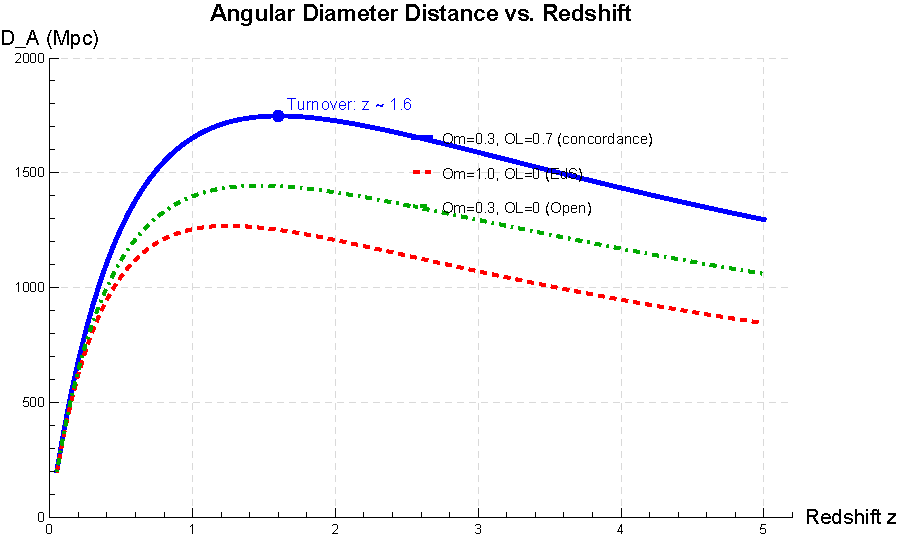
\includegraphics[width=0.75\textwidth]{../Figures/03_Cosmological_Distances/DA_vs_z.pdf}
    \caption{Angular diameter distance $D_A(z)$ for the concordance
    cosmology ($\Omegam = 0.3$, $\OmegaL = 0.7$,
    $\Hubble = 70$~km\,s$^{-1}$\,Mpc$^{-1}$).  $D_A$ reaches a
    maximum of approximately 1748~Mpc at $z \approx 1.6$ and
    then decreases.  This turnover is a key consequence of the
    expanding universe and has no analogue in Euclidean geometry.
    Generated by \texttt{friedmann\_equations.wl}.}
    \label{fig:DA_vs_z}
\end{figure}

\begin{remark}
The turnover of $D_A(z)$ has practical consequences for lensing: a lens
at $z_d \sim 0.5$ and a source at $z_s \sim 2$ might have a
surprisingly large distance ratio $\Dds/\Ds$, and the ``sweet spot''
for lensing efficiency is typically $z_d \sim 0.2$--$0.5$ for sources
at $z_s \sim 1$--$3$.
\end{remark}


% =====================================================================
\section{Luminosity Distance}
\label{sec:luminosity_distance}

The \textbf{luminosity distance} $D_L$ is defined so that the observed
flux $F$ from a source of luminosity $L$ satisfies the Euclidean
inverse-square law:
\begin{equation}
    F = \frac{L}{4\pi D_L^2} \,.
    \label{eq:DL_def}
\end{equation}
In an expanding universe, two effects reduce the observed flux beyond
the $1/r^2$ geometric dilution: (1) photon energies are redshifted by
a factor $(1+z)$, and (2) photon arrival rates are reduced by another
factor $(1+z)$.  This gives:
\begin{equation}
    D_L(z) = (1+z)\, S_k(\chi(z)) = (1+z)^2\, D_A(z) \,.
    \label{eq:DL}
\end{equation}

The relation $D_L = (1+z)^2 D_A$ is the \textbf{Etherington reciprocity
theorem} (or \textbf{distance-duality relation}).  It holds for any
metric theory of gravity in which photons travel on null geodesics and
photon number is conserved.


\begin{derivation}[The two factors of $(1+z)$ in $D_L$]
Flat case.  Photons emitted isotropically now cross a sphere of proper area
$4\pi D_M^2$ around the source (the comoving radius is $D_M = \chi$ and
$a(t_0) = 1$).  Each photon arrives with energy reduced by $1/(1+z)$, and the
arrival rate is reduced by $1/(1+z)$ (time dilation of the emission interval).
So $F = L/[4\pi D_M^2(1+z)^2]$; comparing with eq.~\eqref{eq:DL_def},
$D_L = (1+z)D_M = (1+z)^2D_A$.  Lensing uses only $D_A$; $D_L$ matters when
converting a lensed flux to a luminosity.
\end{derivation}
\begin{figure}[ht]
    \centering
    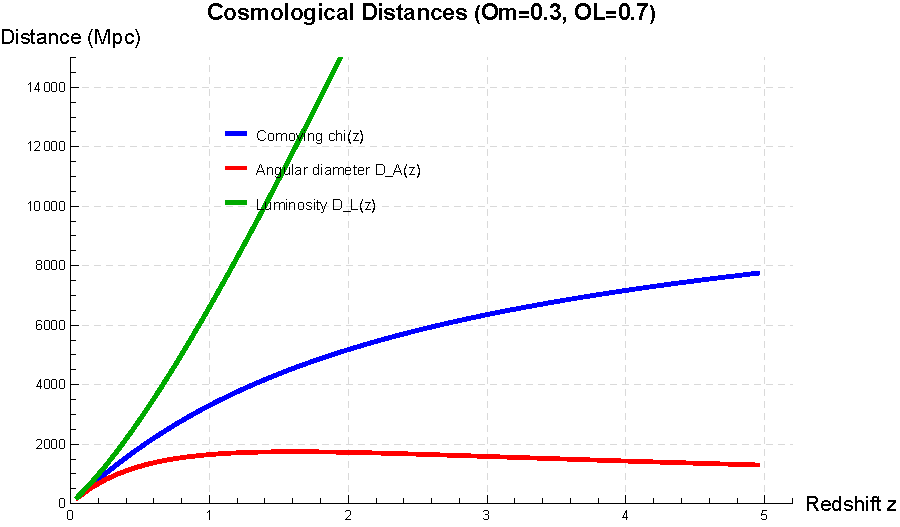
\includegraphics[width=0.75\textwidth]{../Figures/03_Cosmological_Distances/distances_vs_z.pdf}
    \caption{Comoving distance $\chi(z)$ (blue), angular diameter
    distance $D_A(z)$ (red), and luminosity distance $D_L(z)$ (green)
    for the concordance cosmology.  At low redshift ($z \ll 1$) all
    three converge: $\chi \approx D_A \approx D_L \approx
    \speedoflight z / \Hubble$.  At high redshift they diverge
    dramatically.  The turnover of $D_A$ is clearly visible, while
    $D_L$ grows monotonically.  Generated by
    \texttt{friedmann\_equations.wl}.}
    \label{fig:distances_vs_z}
\end{figure}


% =====================================================================
\section{The Lens--Source Angular Diameter Distance}
\label{sec:Dds}

For gravitational lensing, we need not only $\Dd = D_A(z_d)$ and
$\Ds = D_A(z_s)$, but also $\Dds$: the angular diameter distance from
the \textit{lens} to the \textit{source}.  This is \textbf{not} simply
$D_A(z_s) - D_A(z_d)$, because angular diameter distances do not add
linearly.

In a flat universe ($k = 0$), the comoving distances \textit{do} add:
$\chi_{ds} = \chi_s - \chi_d$, and the lens--source angular diameter
distance is:
\begin{equation}
    \boxed{
    \Dds = \frac{\chi_s - \chi_d}{1 + z_s}
    = \frac{1}{1+z_s}\int_{z_d}^{z_s}
    \frac{\speedoflight\, dz'}{H(z')}
    }
    \label{eq:Dds_flat}
\end{equation}
For a general (non-flat) universe one uses the Hogg~(1999) form
(eq.~19; equivalently Congdon \& Keeton eq.~3.155):
\begin{equation}
    \Dds = \frac{1}{1+z_s}\!\left[
    D_M(z_s)\sqrt{1 + \Omega_k\,D_M^2(z_d)/D_H^2}
    - D_M(z_d)\sqrt{1 + \Omega_k\,D_M^2(z_s)/D_H^2}
    \right]\!,
    \label{eq:Dds_general}
\end{equation}
where $D_M(z) = (1+z)\,D_A(z)$ is the transverse comoving distance,
$D_H = \speedoflight/\Hubble$ is the Hubble distance, and
$\Omega_k = -k\,(\speedoflight/(\Hubble R_0))^2$ is the curvature density
parameter.  For the spatially flat case ($\Omega_k = 0$),
eq.~\eqref{eq:Dds_general} reduces to eq.~\eqref{eq:Dds_flat}, which is
exact and sufficient for the rest of these notes.


\begin{derivation}[Eq.~\eqref{eq:Dds_general} is a subtraction formula]
In an open universe ($\Omega_k > 0$) the comoving separation of the two planes is
still $\chi_s - \chi_d$ along the line of sight, and the transverse comoving
distance between them is $R_0\sinh[(\chi_s-\chi_d)/R_0]$ with
$R_0 = D_H/\sqrt{\Omega_k}$.  Expand with
$\sinh(x-y) = \sinh x\cosh y - \cosh x\sinh y$ and use
$\cosh y = \sqrt{1 + \sinh^2 y}$:
\[
  R_0\sinh\frac{\chi_s-\chi_d}{R_0}
  = D_M(z_s)\sqrt{1 + \frac{D_M^2(z_d)}{R_0^2}} - D_M(z_d)\sqrt{1 + \frac{D_M^2(z_s)}{R_0^2}},
\]
with $D_M = R_0\sinh(\chi/R_0)$ and $1/R_0^2 = \Omega_k/D_H^2$ (checks
B10a--b).  Dividing by $1+z_s$ gives eq.~\eqref{eq:Dds_general}.  For a closed
universe the same steps with $\sin$ and $\cos$ give the same formula with
$\Omega_k < 0$ (check B10c).  For $\Omega_k \to 0$ the square roots tend to~1
and the flat result is recovered.
\end{derivation}

\begin{derivation}[The full chain for flat $w_0w_a$CDM: $\chi(z) \to D_A(z_1,z_2)$]
This is the calculation every double-source-plane analysis repeats.  Inputs:
$\Omegam$, $w_0$, $w_a$, $\Hubble$; flatness, so $\Omega_{\rm DE} = 1-\Omegam$.
\begin{enumerate}
  \item Dark-energy density: $\zeta(z) = (1+z)^{3(1+w_0+w_a)}\exp[-3w_az/(1+z)]$
        (CPL annotation in the equation-of-state section).
  \item Expansion rate: $E(z) = \sqrt{\Omegam(1+z)^3 + (1-\Omegam)\zeta(z)}$.
  \item Comoving distance: $\chi(z) = d_H\int_0^z dz'/E(z')$,
        $d_H = \speedoflight/\Hubble$.  One numerical quadrature per redshift.
  \item Flat, so comoving distances along one line of sight add:
        $\chi(z_1,z_2) = \chi(z_2) - \chi(z_1)$.
  \item Angular-diameter distance between the planes:
        $D_A(z_1,z_2) = [\chi(z_2) - \chi(z_1)]/(1+z_2)$; with $z_1 = 0$ this is
        the ordinary $D_A(z_2)$.
\end{enumerate}
In Mathematica, steps 2--5 are three lines:\\
\texttt{EE[z\_] := Sqrt[om (1+z)\^{}3 + (1-om) (1+z)\^{}(3(1+w0+wa)) Exp[-3 wa z/(1+z)]]}\\
\texttt{chi[z\_] := dH NIntegrate[1/EE[x], \{x, 0, z\}]}\\
\texttt{DA[z1\_, z2\_] := (chi[z2] - chi[z1])/(1 + z2)}

\smallskip
\textit{Worked numbers} ($\Omegam = 0.3$, $\Hubble = 70$):
$D_A(0.5, 2.0) = 1097$~Mpc for $(w_0,w_a) = (-1,0)$, reproducing the
$\Lambda$CDM value below; $1072$~Mpc for $(-0.9, 0)$; $1047$~Mpc for
$(-0.9, 0.3)$ (checks B14a--b).  A $0.1$ change in $w_0$ moves a single
distance by about $2\%$.
\end{derivation}
\begin{remark}
A common mistake is to write $\Dds = \Ds - \Dd$.  This is \textbf{wrong}
in general.  Even in a flat universe, $\Dds \neq \Ds - \Dd$ because the
factors of $(1+z)$ are different.  One must always compute $\Dds$ using
eq.~\eqref{eq:Dds_flat} (or its curved-space generalization).  To
illustrate: for $z_d = 0.5$ and $z_s = 2.0$ in the concordance
cosmology, $\Dd \approx 1259$~Mpc, $\Ds \approx 1727$~Mpc, but
$\Dds \approx 1097$~Mpc $\neq \Ds - \Dd \approx 468$~Mpc.
\end{remark}


\begin{annotation}[The subtraction trap, quantified]
In a flat universe the exact relation between $\Dds$ and the naive difference is
\[
  \Dds - (\Ds - \Dd) = \frac{\chi_s - \chi_d}{1+z_s} - \frac{\chi_s}{1+z_s}
  + \frac{\chi_d}{1+z_d}
  = \Dd\,\frac{z_s - z_d}{1+z_s}
  \qquad(\text{check B13c}),
\]
always positive: $\Ds - \Dd$ always \emph{underestimates} $\Dds$.  For the
example above the gap is $1259 \times 1.5/3 = 630$~Mpc (check B13d), more than
the ``answer'' $468$~Mpc itself.  It is not a small correction.

\textit{Order matters.}  $D_A(z_1,z_2)$ is not symmetric:
$D_A(z_2,z_1) = (\chi_2-\chi_1)/(1+z_1) = [(1+z_2)/(1+z_1)]\,D_A(z_1,z_2)$.  For
$z_1 = 0.5$, $z_2 = 2$: $D_A(2\to0.5) = 2194$~Mpc, twice $\Dds$ (check B13b).
Lensing always wants the observer-side redshift first, $\Dds = D_A(z_d,z_s)$.
\end{annotation}

\begin{bridge}[The DSPL ratio is a ratio of comoving distances]
Chapter~\ref{ch:multiplane_dspl} measures
$\Brat = D_{ls_1}D_{s_2}/(D_{s_1}D_{ls_2})$ for a lens at $z_l$ with sources at
$z_{s_1} < z_{s_2}$.  In a flat universe, inserting
$D_A(z_1,z_2) = (\chi_2-\chi_1)/(1+z_2)$ for all four distances, the
$(1+z_{s_1})$ and $(1+z_{s_2})$ factors cancel in pairs:
\[
  \Brat = \frac{(\chi_{s_1} - \chi_l)\,\chi_{s_2}}{\chi_{s_1}\,(\chi_{s_2} - \chi_l)}
  \qquad(\text{check B15a}).
\]
So $\Brat$ depends only on comoving distances, and (since every $\chi$ scales
with $d_H$) not at all on $\Hubble$ (check B15c).  Example:
$z_l = 0.3$, $z_{s_1} = 0.8$, $z_{s_2} = 2.0$, flat $\Lambda$CDM with
$\Omegam = 0.3$ gives $\Brat = 0.743$, comfortably below~1 (check B15b).  Note
how the subtraction trap would enter: using $D_{ls} = D_s - D_l$ would be wrong
in both the numerator and the denominator.
\end{bridge}

\begin{bridge}[How weakly $\Brat$ depends on $w$]
Chapter~\ref{ch:cosmological_sensitivity} needs $\partial\Brat/\partial w$.  For
the example above, a centred finite difference of the full chain gives
$d\ln\Brat/dw_0 = -0.032$ at $w_0 = -1$: moving $w_0$ from $-1$ to $-0.9$
lowers $\Brat$ by only $0.3\%$ (check B15d), much less than the $\approx 2\%$
change of a single distance (previous derivation box), because the dependence on
$w$ largely cancels in the ratio.  This is why DSPL cosmography needs
per-cent-level measurements of $\Brat$ to say anything about $w$.
\end{bridge}

% =====================================================================
\section{The Distance Ratio for Lensing}
\label{sec:distance_ratio}

The \textbf{lens equation} (Module~4) and the \textbf{Einstein radius}
both depend on a specific combination of distances.  The Einstein radius
of a point mass $M$ is (Congdon \& Keeton eq.~2.25):
\begin{equation}
    \thetaE = \sqrt{\frac{4\Gnewton M}{\speedoflight^2}
    \frac{\Dds}{\Dd\,\Ds}}
    \label{eq:einstein_radius_preview}
\end{equation}
and the critical surface mass density is:
\begin{equation}
    \Sigmacr = \frac{\speedoflight^2}{4\pi\Gnewton}
    \frac{\Ds}{\Dd\,\Dds} \,.
    \label{eq:sigma_cr_preview}
\end{equation}

The key quantity is the \textbf{distance ratio}:
\begin{equation}
    \mathcal{D} \equiv \frac{\Dds}{\Dd\,\Ds} \,,
    \label{eq:distance_ratio}
\end{equation}
which determines the ``lensing strength'' of a given observer--lens--source
configuration.

Note that $\mathcal{D}$ is \textit{not} simply $1/\Dd$, because $\Dds$
depends on both $z_d$ and $z_s$ in a non-trivial way.  The distance
ratio is maximized (lensing is most efficient) when the lens is roughly
halfway between the observer and the source in terms of comoving
distance.


\begin{annotation}[Which distance goes where]
\begin{itemize}
  \item $\Dds/\Ds$ converts the physical deflection $\alphahat$ to the
        reduced deflection $\alpha$ seen on the sky.  It lies between 0 (lens
        at the source) and 1 (lens at the observer).
  \item $\Dd$ converts angles in the lens plane to physical lengths,
        $\xi = \Dd\theta$; $\Ds$ does the same in the source plane.
  \item $\Sigmacr = (\speedoflight^2/4\pi\Gnewton)\,\Ds/(\Dd\Dds)$: the
        source distance is upstairs.  A handy numerical form is
        $\Sigmacr = 1.663\times10^{12}\,\Msun\,\text{kpc}^{-2}\times
        [\Ds/(\Dd\Dds)$ in Mpc$^{-1}]$, since
        $\speedoflight^2/4\pi\Gnewton = 1.07\times10^{26}$~kg\,m$^{-1}$
        (checks B17a--b).
  \item $\thetaE = 2.85''\,(M/10^{12}\Msun)^{1/2}\,(\mathcal{D}/\text{Gpc}^{-1})^{1/2}$
        (check B19e).
\end{itemize}

\textit{Careful with ``maximised''.}  At fixed $z_s$, $\mathcal{D} =
\Dds/(\Dd\Ds)$ itself is \emph{not} maximised at intermediate $z_d$: it
diverges as $z_d \to 0$ (where $\Dd \to 0$) and decreases monotonically to zero
at $z_d = z_s$ (check B16d, for $z_s = 1$).  The quantity that peaks at
intermediate $z_d$ is the efficiency $\Dd\Dds/\Ds = \Dd^2\mathcal{D}$ of the next
section, i.e.\ the physical Einstein radius at fixed mass.
\end{annotation}

% =====================================================================
\section{Lensing Efficiency}
\label{sec:lensing_efficiency}

For a fixed source redshift $z_s$, one can ask: at what lens redshift
$z_d$ is lensing most efficient?  The answer is determined by the
\textbf{lensing efficiency function}:
\begin{equation}
    \mathcal{E}(z_d; z_s) \equiv \frac{\Dd\,\Dds}{\Ds}
    \label{eq:lensing_efficiency}
\end{equation}
which is proportional to the square of the Einstein radius (at fixed
mass).  Note that $\thetaE^2 \propto \Dds/(\Dd\,\Ds) =
\mathcal{D}$, while the physical Einstein ring area scales as
$\Dd^2 \thetaE^2 \propto \Dd\,\Dds/\Ds = \mathcal{E}$.

\begin{figure}[ht]
    \centering
    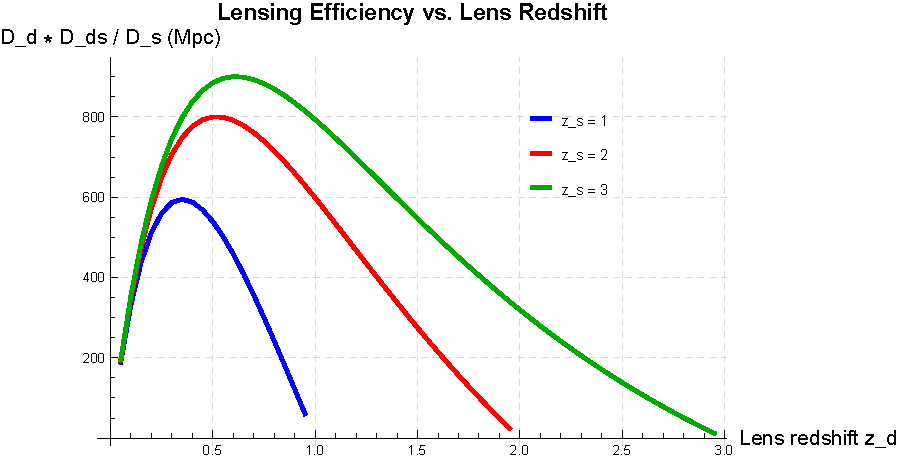
\includegraphics[width=0.75\textwidth]{../Figures/03_Cosmological_Distances/lensing_efficiency.pdf}
    \caption{Lensing efficiency $\Dd\,\Dds/\Ds$ as a function of lens
    redshift $z_d$ for several source redshifts $z_s = 1, 2, 3$ in
    the concordance cosmology.  For $z_s = 1$, lensing is most
    efficient at $z_d \approx 0.35$; for $z_s = 2$, at
    $z_d \approx 0.5$.  The lens is typically most effective when
    placed roughly ``halfway'' (in comoving distance) between the
    observer and the source.  Generated by
    \texttt{friedmann\_equations.wl}.}
    \label{fig:lensing_efficiency}
\end{figure}


\begin{derivation}[Where the efficiency peaks, and why not exactly halfway]
Flat case: $\Dd\Dds/\Ds = \chi_d(\chi_s-\chi_d)/[(1+z_d)\chi_s]$ (check B16b;
the $(1+z_s)$ cancels).  Without the $1/(1+z_d)$ this would be a parabola in
$\chi_d$ peaking exactly at $\chi_d = \chi_s/2$.  The $1/(1+z_d)$ factor
penalises distant lenses and pulls the peak toward the observer: for $z_s = 1$
the maximum is at $z_d = 0.35$, where $\chi_d/\chi_s = 0.42$; for $z_s = 2$ it
is at $z_d = 0.52$ (checks B16a, B16c).
\end{derivation}

% =====================================================================
\section{Summary}
\label{sec:cosmo_summary}

\begin{itemize}
    \item The \textbf{cosmological principle} (homogeneity + isotropy)
          constrains the spacetime metric to the Robertson--Walker form
          $ds^2 = -\speedoflight^2 dt^2 + a^2(t)\left[dr^2/(1-kr^2)
          + r^2 d\Omega^2\right]$.

    \item Plugging the RW metric into \textbf{Einstein's equations} with
          a perfect-fluid stress-energy tensor yields the
          \textbf{Friedmann equations}:
          \begin{align*}
          H^2 &= \frac{8\pi\Gnewton\rho}{3}
          - \frac{k\speedoflight^2}{a^2}
          + \frac{\Lambda\speedoflight^2}{3} \,, \\
          \frac{\ddot{a}}{a} &= -\frac{4\pi\Gnewton}{3}
          \left(\rho + \frac{3p}{\speedoflight^2}\right)
          + \frac{\Lambda\speedoflight^2}{3} \,.
          \end{align*}

    \item The density parameters $\Omegam$, $\OmegaL$, $\Omega_k$
          satisfy $\Omegam + \OmegaL + \Omega_k = 1$ (ignoring
          radiation at late times).

    \item The \textbf{angular diameter distance} $D_A(z) = \chi(z)/(1+z)$
          is \textit{not monotonic}: it turns over at $z \approx 1.6$
          in the concordance cosmology.

    \item The \textbf{luminosity distance} is $D_L = (1+z)^2 D_A$
          (Etherington reciprocity).

    \item The \textbf{lens--source distance} $\Dds \neq \Ds - \Dd$;
          it must be computed as
          $\Dds = (\chi_s - \chi_d)/(1+z_s)$ for a flat universe.

    \item The \textbf{Einstein radius} $\thetaE \propto
          \sqrt{\Dds/(\Dd\,\Ds)}$ depends on the distance configuration,
          and lensing is most efficient when the lens is roughly
          halfway (in comoving distance) to the source.
\end{itemize}


% =====================================================================
\section{Problems}
\label{sec:cosmo_problems}

\begin{exercise}
\label{ex:friedmann_derivation}
\textbf{(Deriving the Friedmann equations from the RW metric.)}
Starting from the Robertson--Walker metric~\eqref{eq:rw_metric}:
\begin{enumerate}[label=(\alph*)]
    \item Compute the Christoffel symbols for the FRW metric.
    \item Compute the Ricci tensor $R_{\mu\nu}$ and Ricci scalar $\ricciS$.
    \item Use Einstein's equations with the perfect-fluid
          stress-energy tensor to derive the first and second
          Friedmann equations.
    \item Show that differentiating the first Friedmann equation and
          using the second gives the fluid conservation equation.
\end{enumerate}
Verify all steps with
\mathlink{03_Cosmological_Distances/friedmann_equations.wl}{friedmann\_equations.wl}.
\end{exercise}

\begin{exercise}
\label{ex:age_of_universe}
\textbf{(Age of the universe for different cosmologies.)}
The age of the universe is
$t_0 = \int_0^\infty dz / [(1+z)\, H(z)]$.
\begin{enumerate}[label=(\alph*)]
    \item For an Einstein--de~Sitter universe ($\Omegam = 1$,
          $\OmegaL = 0$, $k = 0$), show analytically that
          $t_0 = 2/(3\Hubble)$.
    \item Compute $t_0$ numerically for the concordance cosmology
          ($\Omegam = 0.3$, $\OmegaL = 0.7$).  You should find
          $t_0 \approx 13.5$~Gyr for $\Hubble = 70$~km\,s$^{-1}$\,Mpc$^{-1}$.
    \item Compare with an open universe ($\Omegam = 0.3$,
          $\OmegaL = 0$, $\Omega_k = 0.7$).
\end{enumerate}
\end{exercise}

\begin{exercise}
\label{ex:DA_turnover}
\textbf{(Angular diameter distance turnover.)}
\begin{enumerate}[label=(\alph*)]
    \item Plot $D_A(z)$ for the following cosmologies and identify the
          turnover redshift in each:
          (i) $\Omegam = 0.3$, $\OmegaL = 0.7$ (concordance);
          (ii) $\Omegam = 1.0$, $\OmegaL = 0$ (Einstein--de~Sitter);
          (iii) $\Omegam = 0.3$, $\OmegaL = 0$ (open).
    \item Explain physically why $D_A$ turns over: why do high-redshift
          objects appear \textit{larger} than intermediate-redshift objects?
    \item For the concordance cosmology, find the redshift $z_{\max}$
          at which $D_A$ is maximum by numerically solving
          $dD_A/dz = 0$.
\end{enumerate}
\end{exercise}

\begin{exercise}
\label{ex:real_lens}
\textbf{(Distances for a real lens system: Q0957+561.)}
The first gravitational lens discovered (Walsh, Carswell \& Weymann 1979)
has lens redshift $z_d = 0.36$ and source redshift $z_s = 1.41$.
Using the concordance cosmology:
\begin{enumerate}[label=(\alph*)]
    \item Compute $\Dd$, $\Ds$, and $\Dds$ in Mpc.
    \item Verify that $\Dds \neq \Ds - \Dd$.
    \item Compute the critical surface mass density $\Sigmacr$ in
          $\Msun\,\text{kpc}^{-2}$.
    \item Compute the Einstein radius $\thetaE$ for a lens mass
          $M = 10^{12}\,\Msun$.
\end{enumerate}
\end{exercise}

\begin{exercise}
\label{ex:einstein_radius_numerical}
\textbf{(Einstein radius for a typical galaxy lens.)}
For a flat $\Lambda$CDM universe with $\Omegam = 0.3$,
$\OmegaL = 0.7$, $\Hubble = 70$~km\,s$^{-1}$\,Mpc$^{-1}$:
\begin{enumerate}[label=(\alph*)]
    \item Compute $\Dd$, $\Ds$, $\Dds$ for $z_d = 0.3$, $z_s = 1.0$.
    \item Compute the Einstein radius $\thetaE$ for a lens mass
          $M = 10^{12}\,\Msun$.  You should find $\thetaE \approx 2.4''$.
    \item How does $\thetaE$ scale with $M$?  What mass gives
          $\thetaE = 10''$?
    \item Plot $\thetaE$ as a function of $z_d$ (with $z_s = 1$ and
          $M = 10^{12}\,\Msun$ fixed).  Does $\thetaE$ have a maximum?
          At what $z_d$ is the physical Einstein radius
          $\RE = \Dd\thetaE$ largest?
\end{enumerate}
Verify with
\solnlink{03_Cosmological_Distances/problems\_03.wl}{problems\_03.wl}.
\end{exercise}
